\chapter{Proposed approach}
\label{chp:approach}

As previous mentioned, this thesis aims at answering the question of\textit{ how
to support the specification of applications that handle both multimodal
interactions and multiple interacting users} (RQ1). Some researches
~\cite{dumas_description_2010, katsurada_xisl:_2005, w3c_multimodal_2003} in HCI
also address this question, but they suffer from some relevant drawbacks
(discussed in \sect{sec:state:drawbacks}). In particular, they \textit{lack
support for fine
synchronization among modalities}. The specification of output modalities
synchronization is addressed by VMM by studies in multimedia languages. Thus, we
address this question by integrating efforts from both HCI and VMM and we aim at
extending multimedia languages to offer such support.

By so extending multimedia languages, we also aim to answer \textit{how to
extend the output-oriented development in multimedia languages to also handle
these interaction, besides the ordinary GUI-based ones, and multiple interacting
users} (RQ2). This question considers that the state of art suffers from a
drawback of \textit{strong encapsulation between fusion and fission}. More
precisely, multimedia specification approaches delegate the input modalities and
fission process, whereas MUI specification approaches delegate output modalities
and fusion process. Thus, we address this question by proposing a multimedia
document model with a set of entities that multimedia languages should
instantiate.

\fig{fig:model} shows the entities of our proposed model, which are:
\textit{Media} (detailed in \sect{sec:approuach:node}), for defining output
modalities to be presented in audiovisual devices and actuators;
\textit{Recognizer}, for identifying an expected input modality captured from an
input device or sensor (detailed in \sect{sec:approuach:node});
\textit{UserClass}, to enable multiuser interactions and user-based contextual
information (detailed in \sect{sec:approuach:userclass}); and
\textit{Relationship}, which uses causal relationship to combine both input and
output modalities using CARE-compatible conditions (detailed in
\sect{sec:approuach:relationship}).

\begin{figure}[!ht]
\begin{center}
	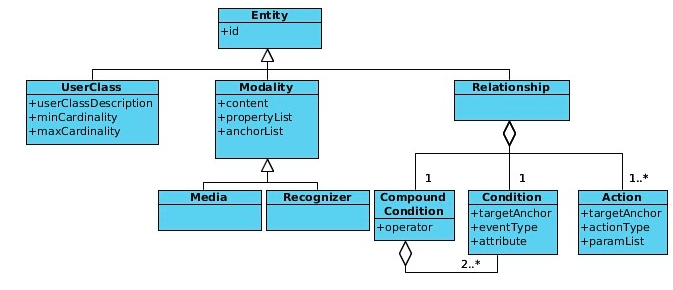
\includegraphics[width=12cm, keepaspectratio]{img/img9.png}
	\caption{Class diagram for the proposed model.}
	\captionvspace
	\label{fig:model}
\end{center}
\end{figure}

The model is based on the NCM entities~\cite{soares_nested_2009}. In particular,
we follow a structure-based~\cite{bolt_put-that-there:_1980} paradigm, which
means that the multimedia document is decoupled from the modalities contents. A
language following our model acts as glue language and does not restrict or
define what kinds of \textit{Media} and
\textit{Recognition} are supported. \fig{fig:shematic} depicts this structure,
in which a
multimedia document should define how \textit{Media}, \textit{Recognition}, and
\textit{UserClass }are related in time, using Relationships, not carrying their
actual contents or descriptions. Then, if one changes the contents of an entity,
from a
\textit{Media}, \textit{Recognizer}, or \textit{UserClass}, this will not change
the document structure. For instance, in the “Put-That-There” scenario, the
speech synthesis can be replaced by a video or the gesture recognition can be
replaced by speech recognition.

\begin{figure}[!ht]
\begin{center}
	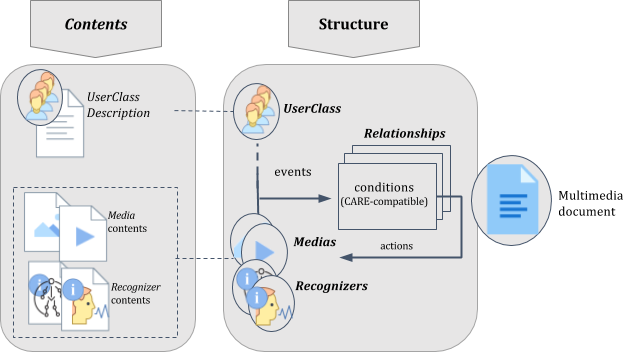
\includegraphics[width=10cm, keepaspectratio]{img/img10.png}
	\caption{Schematic view of the proposed multimedia document.}
	\label{fig:shematic}
    \captionvspace
\end{center}
\end{figure}

The next subsections detail each entity of the model.

\section{Media and Recognizer}
\label{sec:approuach:node} An interaction modality can be specialized in two
main entities: \textit{Media} and
\textit{Recognizer}. It is defined by its Content, a list of \textit{anchor}s,
and a list of \textit{properties}.

\textit{Media} entities are capable of producing output in certain modalities
through audiovisual devices and actuators. For instance, a TTS (Text-To-Speech)
synthesizer produces audio speech to be played through a speaker. Similar to the
recognizer \textit{content}, the media \textit{content} is also decoupled from
the multimedia document and it is referenced by a location property. The media
\textit{content} can be an ordinary audiovisual content —such as audio, video,
image— or a document described in a unimodal synthesizer language, \textit{e.g.} an SSML
file. \textit{Anchor}s are portions of the content presentation. For instance,
an \textit{anchor} may define a temporal portion of a video (\textit{e.g.} a segment of
the video presentation ranging from 30 to 50 seconds). Additionally, an
\textit{Anchor} may refer to the identifier of an internal element in the
synthesizer document, \textit{e.g.} an SSML element to be synthesized. \textit{Properties}
define parameters for \textit{Media}, such as the transparency of video, the
volume of the audio output produced by an SSML speech synthesizer, the frame
rate of a BML avatar rendering animation, etc.

\textit{Recognizer} entities are capable of identifying an expected input in a
certain modality captured from an input device or sensor. For example, an ASR
(Audio Speech Recognition) recognizer identifies sentences in audio samples
captured by a microphone. The \textit{content} of a \textit{Recognizer} is
decoupled from the multimedia document and it is referenced by a location
property (the URL of the content). The content can be a document described in a
unimodal recognizer language, \textit{e.g.} an SRGS file. \textit{anchor}s are portions
of the recognizer content. They define when or what to expect, within a
document, a certain input modality to be recognized. For instance, an SRGS
defines one rule element for each expected speech input (\textit{e.g.} a certain rule may
define that acceptable input tokens are “put that” and “there”). An anchor
enables the multimedia document to know the moment when the recognition of a
token is complete. \textit{Propertie}s define parameters for the
\textit{Recognizer} or dynamic values inside the \textit{Recognizer}. For
example, an ink recognizer can have properties to indicate the current position
of the ink pointer.

\section{UserClass}
\label{sec:approuach:userclass}

In multiuser applications, a user may assume different roles. For instance, it
is possible to create an application that behaves differently if the user is a
professor or a student. Moreover, both professors and students can use the
application at the same time. By supporting multiuser features in the authoring
model, a developer can create applications that are aware of the users who are
interacting with them, and how. To support multiuser features, the
\textit{UserClass} is used to model the different types of interacting users,
\textit{i.e.}~different roles that users can play when using an application.

A \textit{UserClass} is defined by its \textit{minCardinality} and
\textit{maxCardinality} attributes, and by a \textit{userClassDescription}. The
id attribute uniquely defines a UserClass. The cardinality attributes allow us
to limit the number of users that can be part of that \textit{UserClass}. The
\textit{userClassDescription} specifies how users are identified as being part
of the \textit{UserClass}. To do that, each user who can interact with the
system must have a \textit{profile description}. The user profile may include,
for example, information such as whether he/she is a student or a professor.
Moreover, it may include the devices he/she is using to interact with the
application. The \textit{userClassDescription} then should specify which users,
based on their profiles, are part of each \textit{UserClass}.

Note that the specification of \textit{userClassDescription} is tied to the
specific vocabulary used to describe the user’s profiles. Our model is agnostic
and does not prescribe the \textit{userClassDescription} specification details,
which should be defined by the language instantiation. For instance, we propose
in our language instantiations (discussed in \chp{chp:instantiation}) the use
of an RDF description for user
\textit{profile description }and \textit{SPARQL}, which enables queries over RDF
entities, for
\textit{userClassDescription}.

Runtime properties related to users in a \textit{UserClass}, such as the number
of users registered in a class and user context, should be stored as global
variables. In particular, regarding the user context, the language must support
the description of human sensory capabilities, which can be used during modality
selection. Examples of such variables are \textit{canHear}, \textit{canSee}, and
\textit{canSpeak}. Therefore, a modality selection can be specified through
conditional control structures, such as \textit{switch }or
\textit{if-then-else}, which evaluate these runtime properties.

\tab{table:selection} shows examples of modality selection considering users’
sensory capabilities.\footnote{The recommendation of modalities given users’
sensory capabilities should draw on accessibility research results.
\tab{table:selection} is simply an illustration that our approach makes it
feasible to build MUIs considering those capabilities.} For instance, when the
\textit{canSee} variable is
\textit{false}, audio or speech modalities should be used instead of visual and
GUI modalities; and when \textit{canHear} is \textit{false} an avatar-based
modality should be selected instead of audio modalities.

\begin{table}
\setlist[itemize]{topsep=0pt}
\scriptsize
\def\arraystretch{1.5}
\begin{tabular}[!ht]{ c m{5.5cm} m{5.5cm}}

	\hline
	\textbf{Variables} &
	\centering\arraybackslash \textbf{When false} &
	\centering\arraybackslash \textbf{When true} \\
	\hline

	canSee &
	\begin{itemize}
		\item Audio modalities \newline (\textit{e.g.} audio/*)
		\item Speech modalities \newline (\textit{e.g.} SRGS, SSML)
	\end{itemize}
	&
	\begin{itemize}
		\item Visual modalities (\textit{e.g.} \newline video/* img/*, text/plain)
		\item GUI modalities (\textit{e.g.} key presses, mouse
	\end{itemize} \\
	\hline

	canHear &
	\begin{itemize}
		\item Avatar modalities \newline (\textit{e.g.} BML)
	\end{itemize}
	&
	\begin{itemize}
		\item Audio modalities \newline (\textit{e.g.} audio/*)
	\end{itemize}\\
	\hline

	canSpeak &
	\begin{itemize}
		\item Audio modalities \newline (\textit{e.g.} audio/*)
	\end{itemize}
	&
	\begin{itemize}
		\item Speech modalities \newline (\textit{e.g.} SRGS, SSML)
	\end{itemize}\\
	\hline

\end{tabular}
\caption{Examples of modality selection.}
\label{table:selection}
\end{table}

This thesis focuses on specification issues of multiuser interactions. More
precisely, we focus on how the author defines user interaction requirements and
uses context information. We do not directly address, nor prescribe, how the
multimedia system should gather the users’ \textit{profile description} and
retrieval of their runtime context variables. These tasks can be achieved by
explicit user identification (\textit{e.g.} via log in) or by recognition techniques using
sensors (\textit{e.g.} via facial recognition).

\section{Relationship}
\label{sec:approuach:relationship}

\textit{Relationship} entities enable developers to express the combined use of
the modalities perceived by users through \textit{Media} and the modalities
generated by users through \textit{Recognizers}. In the “Put-That-There”
scenario, for instance, Relationship entities express the combined use of speech
syntheses and visual objects (\textit{Media}) with the speech and gesture
recognition (\textit{Recognizers}).
\textit{Relationship} entities are defined by a set of \textit{conditions} and
\textit{actions}. When the
\textit{conditions} are satisfied, then the \textit{actions} are performed. The
actions and
\textit{conditions} in a \textit{Relationship} are detailed as follows.

Regarding the \textit{actions} of the \textit{Relationship}, they enable
developers to change the properties and to control the activation/deactivation
of \textit{Recognizers} and \textit{Medias}. A \textit{set} action changes the
value of a property. Four actions can manipulate the activation/deactivation of
\textit{Recognizers} and \textit{Media}: \textit{start}, which activates a
recognizer or synthesizer; \textit{stop}, which deactivates a
\textit{Recognizer} or \textit{Media} and releases its resources;
\textit{pause}, which deactivates a \textit{Recognizer} or \textit{Media}, but
does not release its resources; and \textit{resume}, which reactivates a
previously paused \textit{Recognizer} or \textit{Media}.
\tab{table:relationship} presents the semantics of those actions over
\textit{Recognizers}, \textit{Media}, and their \textit{anchors}.

In a \textit{Recognizer}, the activation of an anchor “a1” means that the
portion of the
\textit{Recognizer} content related to “a1” is enabled to be recognized. By
default, activating a \textit{Recognizer} without specifying a specific
\textit{anchor} is equivalent to activating all of its \textit{anchor}s. The
recognition of the \textit{anchor} content itself only occurs when the
\textit{Recognizer} identifies the required pattern in the user input in the
corresponding modality. For instance, consider a speech recognizer that defines
two anchors, for the tokens “put that” and “there”. When the recognizer is
activated without specifying an anchor, both anchors are activated and, thus,
either one can be recognized in the audio input (\textit{e.g.} captured by a
microphone).
Moreover, the developer can restrict the recognizable content by starting the
anchors individually.

\begin{table}[H]
\scriptsize
\def\arraystretch{1.5}
\begin{tabular}[!ht]{ m{1cm} m{4.5cm} m{7cm} }
	%%%%%%
	\hline
	\textbf{Action} & \textbf{Over}
		& \textbf{Semantics} \\

	%%%%%%
	\hline
	\multirow{7}{*}{start}
	& \textit{Media} &\textit{Media} starts rendering its content from the beginning.\\
	\cline{2-3}
	& An anchor of a \textit{Media} &	\textit{Media} starts rendering its
	content from that specific anchor. \\
	\cline{2-3}
	& \textit{Recognizer} &	\textit{Recognizer} is activated and it is able to
	recognize all of the anchors of the recognizer content. \\
	\cline{2-3}
	& An anchor of a \textit{Recognizer} &	\textit{Recognizer} is activated
	and it is able to recognize only the content related to that specific
	anchor. \\
	\hline

	%%%%%%
	\multirow{6}{*}{stop}
	& \textit{Media} & \textit{Media} stops rendering its content.\\
	\cline{2-3}
	& An anchor of a \textit{Media} &	\textit{Media} stops rendering the
	content of that specific anchor. \\
	\cline{2-3}
	& \textit{Recognizer} &	\textit{Recognizer} is deactivated and it is unable
	to recognize any content. \\
	\cline{2-3}
	& An anchor of a \textit{Recognizer} &	\textit{Recognizer} is deactivated
	and it is unable to recognize the content related to that specific anchor.\\
	\hline

	%%%%%%
	\multirow{5}{*}{pause}
	& \textit{Media} &	\textit{Media} pauses rendering/synthesizing its
	content, but
	the system does not release its resources.\\
	\cline{2-3}
	& An anchor of a \textit{Media} &	\textit{Media} pauses
	rendering/synthesizing its
	content from that specific anchor, but the system does not release the
	synthesizer’s resources. \\
	\cline{2-3}
	& \textit{Recognizer} / anchor of a \textit{Recognizer} &	Acts as stop. \\
	\hline

	%%%%%%
	\multirow{5}{*}{resume}
	& \textit{Media} &	\textit{Media} restarts rendering/synthesizing its
	content from
	the previously paused state. \\
	\cline{2-3}
	& \textit{Recognizer} &	\textit{Media} restarts rendering/synthesizing its
	content
	from the previously paused anchor. \\
	\cline{2-3}
	& \textit{Recognizer} / anchor of a \textit{Recognizer} &	Acts as start. \\
	\hline
\end{tabular}
%}
\caption{Semantics of the actions over media, recognizers, and their anchors.}
\label{table:relationship}
\end{table}

In a \textit{Media}, the activation of an anchor means that the \textit{Media}
is rendering the content related to that \textit{anchor}. While a synthesizer is
activated and being rendered, its anchors are automatically
activated/deactivated as the presentation content of the \textit{Media} reaches
the content portion related to each
\textit{Anchor}. For instance, consider an \textit{anchor} “a1” of an
audiovisual media “m1” from 300 to 360 seconds. This \textit{Anchor} will be
automatically activated when the presentation of “m1” reaches 300 seconds, and
deactivated when it reaches 360 seconds. This behavior is similar to other types
of \textit{Media}. For instance, consider an \textit{anchor} “a2” that points to
a specific token of an SSML document associated to \textit{Media} “s1”. In
this case, when the presentation of the SMML document —\textit{i.e.}~the speech
synthesis— reaches the token related to “a2”, then “a2” is activated.

A \textit{condition} may test:

\begin{itemize}
	\item the activation of \textit{Recognizers} and \textit{Media}, or their
	anchors. For instance, we can define a \textit{Relationship} to be triggered
	when a (portion of a) video is activated with given attributes;
	\item the recognition of portions of the \textit{Recognizer} content. For
	instance, we can define a \textit{Relationship} to be triggered when the
	recognition of “hello”, defined in an SRGS file, is complete;
	\item values of properties of \textit{Recognizer} or \textit{Media} and
	runtime of a user’s context. For these value tests, the multimedia language
	must provide comparators, such as: is equal to, greater than, and less than.
	For instance, we can define a Relationship to be triggered when the volume of a video becomes greater than 70\% or when the \textit{canHear} value is equal to “false”.
\end{itemize}

\textit{CompoundCondition}s specify the combined use of \textit{conditions} over
the modalities. For instance, a \textit{Relationship} can be defined to be
triggered when portions of a video are activated and the recognition of a
sentence is complete. The following operators are proposed here:

\begin{itemize}
	\item \textit{or}: the \textit{Relationship} will trigger when any one of the
	conditions is satisfied;
	\item \textit{and}: the \textit{Relationship} will trigger when all the
	conditions are satisfied, independently of the order in which they are
	satisfied;
	\item \textit{seq}: the \textit{Relationship} will trigger when all the
	conditions are satisfied in the specified order. This operator was not present in the relationship entity of NCM.
\end{itemize}

\begin{table}[b!]
\scriptsize
\def\arraystretch{1.3}
\begin{tabular}{ m{4cm} m{4.5cm} m{4.5cm}}
	%%%%%%
	\hline
	\textbf{CARE properties} & \textbf{Relationship operators \newline (our approach)} & \textbf{SMUIML transition operators} \\
	\hline

	%%%%%%
	\textbf{Equivalence} &	Compound condition using the or operator &
	Recognizers
	trigger using the seq\_or operator \\
	\hline
	\textbf{Assignment} &	A simple condition &	Only one trigger \\
	\hline
	\textbf{Redundancy (use temporal window)} & Compound condition using the or
	operator
	and activated within a temporal window &	Recognizers trigger using the
	par\_or operator \\
	\hline
	\textbf{Sequential complementarity} & Compound condition using the seq
	operator &
	Recognizers trigger using the seq\_and operator \\
	\hline
	\textbf{Parallel complementarity (use temporal window)} & Compound
	condition using
	the and operator and activated within a temporal window &	Recognizers
	trigger using the par\_and operator \\
	\hline

\end{tabular}
\caption{Expressiveness of the multimodal \textit{Relationship} operators
compared to
SMUIML.}
\label{table:care}
\end{table}

Indeed, the combination of interaction modalities is an important feature of
MUIs. To analyze the expressiveness of the proposed operators,
\tab{table:care} compares them to the CARE properties. \textit{Equivalence} can
be expressed by a compound condition using the or operator. \textit{Assignment}
can be expressed by a simple condition. \textit{Redundancy} can be expressed by
compound conditions using the \textit{or} operator defined within a temporal
window. The temporal window may be defined by activating/deactivating modalities
within a specific period of time.
\textit{Sequential complementarity} is expressed by a compound condition using
the \textit{seq} operator. Finally, \textit{parallel complementarity} is
expressed by a compound condition using the \textit{and} operator defined within
a temporal window. As highlighted in \tab{table:care}, the proposed operators
have the same expressiveness as the CARE properties and SMUIML operators.
However, CARE properties and SMUIML operators consider only input modalities,
whereas our approach supports simple and compound conditions relating any
combination of input and output modalities. In addition, our proposal supports
conditions for evaluating the user’s context.

To support multiuser-oriented development, the recognition \textit{condition} in
a \textit{Relationship} can be parameterized with a “user\_id” attribute. The
value of this attribute defines which specific user from a \textit{UserClass}
can be responsible for generating the event. By doing this, it is possible to
limit which specific users can trigger a \textit{Relationship}. Moreover, we
define another optional attribute in conditions, called “excluded\_user\_id”. In this attribute, developers can define a list of users who are not allowed to
trigger a condition.

\section{Discussion}
\label{sec:approuch:discussion}

We argue in this thesis, that an multimedia language that instate our entities will support both multimodal and multiuser interactions. We believe that these extensions can contribute to the state of the art by overcoming the drawbacks and same time increase multimodal specification expressiveness.

We handled the lack of support for fine synchronization among modalities mainly
by reusing the multimedia players’ infrastructure, which keeps media object
presentations finely synchronized. In our approach, the multimedia language and
its player should also handle recognizers for input events, in the same
infrastructure. The recognizers are responsible for interacting with the user
input devices and sensors, and for triggering anchor events that enable
synchronization by the multimedia player.

Regarding the strong encapsulation between fusion and fission, we solved this
issue by using a structure-based~\cite{bulterman_structured_2005} paradigm and
using the NCM anchor concept. In addition, we have extended this concept to be
used not only by output modalities (\textit{e.g.} instantiated as <media> in NCL), but
also by input modalities (<input>). By so doing, the multimedia document is
decoupled from the content for recognizers and synthesizers. If necessary,
however, the internal behavior of those recognizers and synthesizers can be
known and controlled by the multimedia application through their anchor events.
Conversely, the languages and frameworks discussed in \chp{chp:approach}
delegate one of
them to another entity. For instance, SMUIML sends ad-hoc messages to a
HephaticsTK framework client.

To solve the lack of support for modality selection considering sensory
capabilities, the framework uses context variables that are able to express user
capabilities. Those variables could be used in conditional constructions to
enable the right modality selection based on the user’s sensory capabilities.

Finally, we overcame the interacting users are second-class citizens through
enabling the specification of interacting users, and the association of a user
with recognition events.

Besides overcoming the above drawbacks, our proposal also achieves more
expressiveness when combining both output and input modalities. It does so by
using the causal relationship and anchor concepts from NCM. Those concepts
enable NCM express Allen’s temporal relations among output modalities. In our
approach, we enable such concepts for input modalities which enable it express
Allen’s temporal relations among both output modalities and input modalities.